\documentclass[ % the name of the author
                author={Ainsley Rutterford},
                % the name of the supervisor
                supervisor={Dr. Tilo Burghardt},
                % the degree programme
                degree={MEng},
                % the dissertation    title (which cannot be blank)
                title={Volumetric Coral Analysis using Deep Learning},
                % the dissertation subtitle (which can    be blank)
                subtitle={},
                % the dissertation     type
                type={research},
                % the year of submission
                year={2020} ]{dissertation}

\usepackage{pgfplots}
\pgfplotsset{compat=1.16}
\pgfplotsset{colormap={cool2}{rgb255(0cm)=(255,210,110); rgb255(1cm)=(225,80,49);}}
\pgfplotsset{colormap={cool1}{rgb255(0cm)=(255,255,255); rgb255(1cm)=(255,0,255);}}
\pgfplotsset{major grid style = {dashed}}
\usepackage{lipsum}
\usepackage[parfill]{parskip}
\usepackage{subcaption}
\usepackage{xurl}
\usepackage{xfrac}
\usetikzlibrary{decorations.markings}

\def\ConvColor{rgb:yellow,5;red,2.5;white,5}
\def\ConvReluColor{rgb:yellow,5;red,5;white,5}
\def\PoolColor{rgb:red,1;black,0.3}
\def\UnpoolColor{rgb:blue,2;green,1;black,0.3}
\def\FcColor{rgb:blue,5;red,2.5;white,5}
\def\FcReluColor{rgb:blue,5;red,5;white,4}
\def\SoftmaxColor{rgb:magenta,5;black,7}
\def\ConvColorThree{rgb:blue,9;green,1;white,4}
\def\ReshapeColor{rgb:blue,4;red,2;white,18}

\usepackage{listings}
\usepackage{xcolor}
\usepackage{textcomp} % Allow straight quotes in listings
\usepackage{booktabs}

\RequirePackage[font=small]{caption}

\definecolor{codegreen}{rgb}{0.6,0.6,0.6}
\definecolor{codegray}{rgb}{0.5,0.5,0.5}
\definecolor{codepurple}{rgb}{0.58,0,0.82}
\definecolor{backcolour}{rgb}{0.97,0.97,0.99}
\definecolor{keycolour}{rgb}{0.10,0.20,0.99}

\lstdefinestyle{mystyle}{
    backgroundcolor=\color{backcolour},
    commentstyle=\color{codegreen},
    keywordstyle=\color{keycolour},
    numberstyle=\scriptsize\color{codegray},
    stringstyle=\color{codepurple},
    basicstyle=\ttfamily\small,
    breakatwhitespace=false,         
    breaklines=true,                 
    captionpos=b,                    
    keepspaces=true,                 
    numbers=left,                   
    numbersep=5pt,                  
    showspaces=false,                
    showstringspaces=false,
    showtabs=false,                  
    tabsize=4
}
 
\lstset{style=mystyle}

\begin{document}

% This macro creates the standard UoB title page by using information drawn
% from the document class (meaning it is vital you select the correct degree 
% title and so on).

\maketitle

% After the title page (which is a special case in that it is not numbered)
% comes the front matter or preliminaries; this macro signals the start of
% such content, meaning the pages are numbered with Roman numerals.

\frontmatter

% This macro creates the standard UoB declaration; on the printed hard-copy,
% this must be physically signed by the author in the space indicated.

\makedecl

% LaTeX automatically generates a table of contents, plus associated lists 
% of figures, tables and algorithms.  The former is a compulsory part of the
% dissertation, but if you do not require the latter they can be suppressed
% by simply commenting out the associated macro.

\tableofcontents
% \listoffigures
% \listoftables
% \listofalgorithms
% \lstlistoflistings

\chapter*{Executive Summary}
% {\bf A compulsory section, of at most $1$ page} 
% \vspace{1cm} 

% \noindent
% This section should pr\'{e}cis the project context, aims and objectives,
% and main contributions (e.g., deliverables) and achievements; the same 
% section may be called an abstract elsewhere.  The goal is to ensure the 
% reader is clear about what the topic is, what you have done within this 
% topic, {\em and} what your view of the outcome is.

% The former aspects should be guided by your specification: essentially 
% this section is a (very) short version of what is typically the first 
% chapter.  Note that for research-type projects, this {\bf must} include 
% a clear research hypothesis.  This will obviously differ significantly
% for each project, but an example might be as follows:

% \begin{quote}
% My research hypothesis is that a suitable genetic algorithm will yield
% more accurate results (when applied to the standard ACME data set) than 
% the algorithm proposed by Jones and Smith, while also executing in less
% time.
% \end{quote}

% \noindent
% The latter aspects should (ideally) be presented as a concise, factual 
% bullet point list.  Again the points will differ for each project, but 
% an might be as follows:

% \begin{quote}
% \noindent
% \begin{itemize}
% \item I spent $120$ hours collecting material on and learning about the 
%       Java garbage-collection sub-system. 
% \item I wrote a total of $5000$ lines of source code, comprising a Linux 
%       device driver for a robot (in C) and a GUI (in Java) that is 
%       used to control it.
% \item I designed a new algorithm for computing the non-linear mapping 
%       from A-space to B-space using a genetic algorithm, see page $17$.
% \item I implemented a version of the algorithm proposed by Jones and 
%       Smith in [6], see page $12$, corrected a mistake in it, and 
%       compared the results with several alternatives.
% \end{itemize}
% \end{quote}

This project is concerned with the use of deep learning to automate the estimation of the amount of annual skeletal matter produced by corals.

First, the process of labelling density bands present in two dimensional slices is automated. This is achieved using a convolutional neural network based off of the U-Net architecture~\cite{ronneberger2015u}. To train this network, a dataset containing ${\sim}600$ images was curated from slices extracted from seven individual coral samples. Various data augmentation techniques were also used to artificially expand the dataset. To measure performance, an accuracy metric based off of the Hausdorff distance between the predicted and ground truth boundaries is used. This initial architecture achieved an average Hausdorff distance of 1.X pixels.

Second, the process of labelling density bands present in three dimensions is explored. To this end, the U-Net architecture is modified to process three dimensional data. A larger dataset of manually labelled adjacent slices was curated to train this network containing ${\sim}X$ images extracted from $X$ coral samples.

Finally, once the density bands are identified, the estimation of the distance between the bands is automated using various techniques. These distances are then used to automatically estimate the volume of skeletal matter produced annually.

\section*{Summary of Achievements}

\begin{itemize}
    \item I spent 25 hours manually labelling coral data.
    \item I generated a 2D dataset containing ${\sim}600$ images and a 3D dataset containing ${\sim}X$ images using various scripts I wrote.
    \item Having not taken the ``Deep Learning'' unit, I spent 20 hours researching and learning about the field of deep learning.
    \item I learned how to use the Keras and TensorFlow libraries in order to implement the networks used.
    \item I modified an existing 2D U-Net implementation and trained it on the curated dataset.
    \item I extended the U-Net architecture to process 3D data.
    \item I wrote a ``data generator'' from scratch in Python to allow the input of 3D data into the network since Keras does not have its own implementation.
    \item I implemented online data augmentation of the 3D data.
    \item I implemented a custom accuracy metric in C and wrapped it in a Python function to achieve a ${\sim}315$ times speed up allowing the accuracy to be calculated in minutes rather than hours.
    \item I performed hyper parameter optimisation in order to maximise the performance achieved by the various architectures.
    \item ablation studies too trained the network over 100 times
\end{itemize}

\chapter*{Supporting Technologies}
% {\bf A compulsory section, of at most $1$ page}
% \vspace{1cm} 

% \noindent
% This section should present a detailed summary, in bullet point form, 
% of any third-party resources (e.g., hardware and software components) 
% used during the project.  Use of such resources is always perfectly 
% acceptable: the goal of this section is simply to be clear about how
% and where they are used, so that a clear assessment of your work can
% result.  The content can focus on the project topic itself (rather,
% for example, than including ``I used \mbox{\LaTeX} to prepare my 
% dissertation''); an example is as follows:

% \begin{quote}
% \noindent
% \begin{itemize}
% \item I used the Java {\tt BigInteger} class to support my implementation 
%       of RSA.
% \item I used a parts of the OpenCV computer vision library to capture 
%       images from a camera, and for various standard operations (e.g., 
%       threshold, edge detection).
% \item I used an FPGA device supplied by the Department, and altered it 
%       to support an open-source UART core obtained from 
%       \url{http://opencores.org/}.
% \item The web-interface component of my system was implemented by 
%       extending the open-source WordPress software available from
%       \url{http://wordpress.org/}.
% \end{itemize}
% \end{quote}

\begin{itemize}
\item Avizo
\item GIMP
\item Keras
\item TensorFlow
\item OpenCV
\item Isambard
\item BlueCrystal Phase 4
\end{itemize}

% \chapter*{Notation and Acronyms}
\chapter*{Acronyms}
\begin{tabular}{lcl}
ANN                 &:     & Artificial Neural Network \\
CCA                 &:     & Connected Component Analysis \\
CNN                 &:     & Convolutional Neural Network \\
CPU                 &:     & Central Processing Unit \\
CR                  &:     & Calcification Rate \\
CT                  &:     & Computed Tomography \\
GAN                 &:     & Generative Aversarial Network \\
GIMP                &:     & GNU Image Manipulation Program \\
GPU                 &:     & Graphics Processing Unit \\
LER                 &:     & Linear Extension Rate \\
ReLU                &:     & Rectified Linear Unit \\
SGD                 &:     & Stochastic Gradient Descent \\
\end{tabular}

\chapter*{Acknowledgements}
I am extremely grateful to Dr Tilo Burghardt whose enthusiasm, support, and guidance throughout this project has been invaluable. I will always be thankful for his contributions throughout my entire degree. I would like to extend my sincere thanks to Dr Erica Hendy and Dr Kenneth Johnson for their expertise and enthusiasm for the project. I am also grateful to Leonardo for the time and effort he put into labelling data for this project as well as his consistent support throughout.

\mainmatter

\chapter{Contextual Background}
\label{chap:context}
This chapter outlines and motivates the main objectives of the project. First, the importance of the analysis of coral skeletons is discussed. Next, the motivations for an automated analysis process are outlined and the choice of a deep learning based solution is justified. The challenges involved in completing the project are highlighted, and related works in the analysis of coral skeletons are then briefly discussed. Finally, the main objectives of the project are summarised and listed.

\section{Introduction}

Coral polyps are tiny soft-bodied organisms. Through a process known as calcification, they use calcium and carbonate ions from the surrounding seawater to build themselves hard calcium carbonate skeletons. These polyps reproduce asexually and can form colonies of up to thousands of individual polyps all contributing to the same connected skeleton.

Using X-radiographs in 1972, Knutson et al.\ were able to confirm the presence of annual density bands in these calcium carbonate skeletons~\cite{knutson}. An annual density band consists of two portions: a high-density portion produced during the late summer and a low density portion formed during periods of seasonally lower water temperatures~\cite{highlow}. These bandings are parallel to the growth surface and orthogonal to the direction of growth; examples are shown in Figure \ref{fig:densityexample}. With knowledge of a coral sample's date of collection, these annual band pairs can be counted back through time to provide not only an age of the sample, but also a chronology of the coral's growth. More specifically, the annual banding can be used to measure three aspects of coral growth~\cite{lough2011new}:

\begin{enumerate}
    \item The linear extension rate (mm y$^{-1}$): the distance that the coral grows per year.
    \item The density (g cm$^{-3}$): the density of the skeletal matter being produced.
    \item The calcification rate (g cm$^{-2}$ y$^{-1}$): the mass of skeletal matter being produced per year, calculated by multiplying the linear extension rate with the density.
\end{enumerate}

Analysis of these aspects of growth can be used to determine changes in a coral colony's environmental conditions as it was growing. Lough and Cooper highlight one significant potential use of the banding information contained within coral skeletons: ``skeletal material contained deep within massive corals can be extracted to allow comparisons of present day growth rates with those pre-dating the industrial revolution and hence examine the consequences of climate and environmental changes on coral reefs''~\cite{lough2011new}.

This project aims to automate the estimation of the linear extension rate which can then be used to estimate the calcification rate. Deep learning will be used to extract the boundaries of each annual density band, and the distance between these boundaries will then be estimated using a method based off of the Euclidean distances between points on the boundaries.

\begin{figure}[t]
    \centering
    \begin{subfigure}[t]{0.49\textwidth}
        \centering
        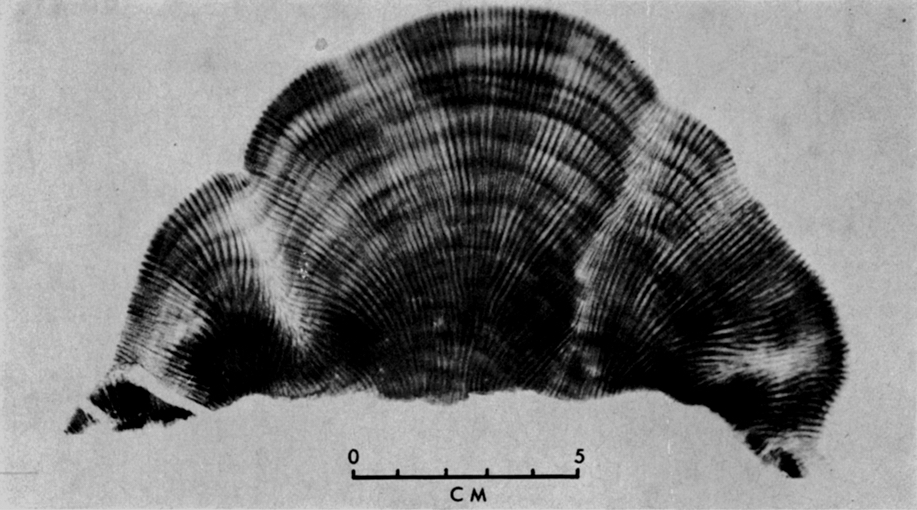
\includegraphics[width=1\textwidth, valign=c]{images/knutson.jpg}
    \end{subfigure}
    ~
    \begin{subfigure}[t]{0.49\textwidth}
        \centering
        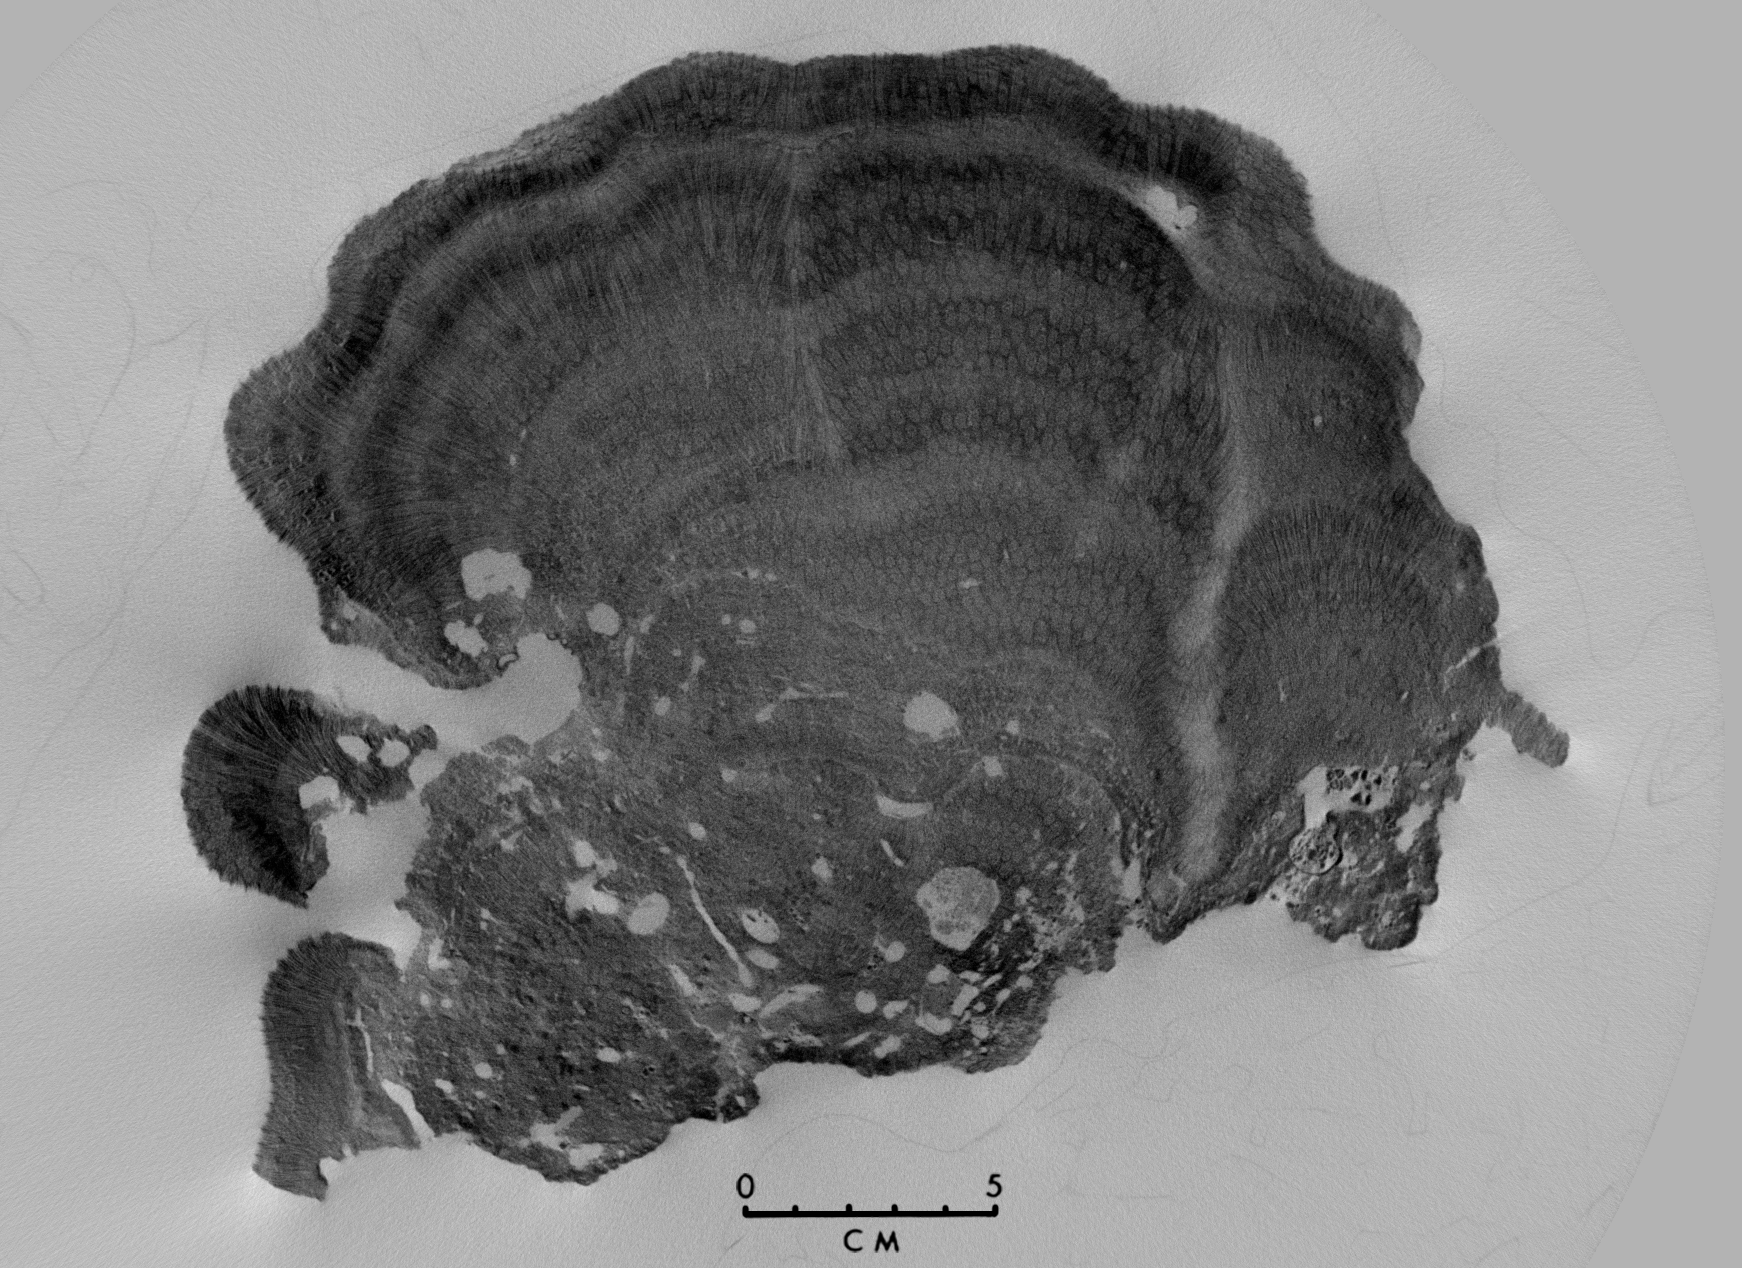
\includegraphics[width=1\textwidth, valign=c]{images/our-coral.png}
    \end{subfigure}
    \caption{Examples of the annual density bands present in the skeletons of a genus of coral called Porites. \textbf{(left)} An X-radiograph of a Porites lobata coral sample presented by Buddemeier, Maragos, and Knutson in 1974: ``[this is a] positive print of the X-ray negative; dark images correspond to high skeletal density, light images to low density''~\cite{coralimage}. \textbf{(right)} An image taken from a CT scan of a Porites sample that exists in the dataset used throughout this project. The image channel has been inverted resulting in dark pixels corresponding to high density, and light pixels corresponding to low density.}
    \label{fig:densityexample}
\end{figure}

\section{Motivations}

% This section discusses the need for an automated solution and attempts to justify the choice of a deep learning based solution.

\subsection{An Automated Solution}

Although many methods for manually estimating the linear extension and calcification rates exist, an automated solution could be beneficial for multiple reasons.

Firstly, opinions on the positions of a particular boundary between high and low density bands can differ from person to person. It is important to note that an idealised annual density cycle is actually in the form of a sinusoidal wave, with the density gradually changing from high to low and back over the course of a year~\cite[p. 39]{coralsine}. Thus, an exact boundary between a high and low band does not actually exist. However, an effort can be made to consistently choose boundaries at the same point in the sinusoid each year. Naturally, people can disagree with each other when determining the positions of the boundaries; a researcher labelling the same slice for a second time might even disagree with their previous choices of boundary positions. This is not the case, however, for an artificial neural network. Once trained, a neural network is deterministic; given a particular input, it will always produce the same output.

Another benefit of the proposed automated solution is speed. An example of a manual solution is to manually label the density boundaries, use a tool to measure distances between multiple points along these boundaries, and average the distances measured to produce a single average linear extension rate. This process can be time consuming. The proposed solution could potentially estimate the calcification rate of a given slice in a matter of seconds. This would allow researchers to not only analyse the density banding quicker, but also ultimately enable them to process more data overall.

Finally, an automated solution has the potential to be more accurate than a manual solution. For example, an automated solution could measure hundreds of distances between two boundaries which could be used to produce a more accurate estimate than a manual solution in which only tens of distances were averaged.

\subsection{Deep Learning}
\label{sec:contextdl}

Feed-forward artificial neural networks have existed in some form since 1965~\cite{deepoverview, 1966cybernetic}, but the term ``deep learning'' was only coined in 2006~\cite{deepoverview, hintondeep, hintonfast}. In the years since, the field of deep learning has seen a significant rise in both its popularity and practicality for a multitude of reasons and is now the state-of-the-art in many areas. This section outlines the justifications of the choice of a deep learning based solution. Deep learning is discussed in more technical detail in Section \ref{sec:deeplearning}.

\subsubsection{The Dataset}

This project will make use of a dataset of more than 160 three dimensional computed tomography (CT) scans of unique coral skeletons from the Natural History Museum's collection. These three dimensional scans are stored as stacks of two dimensional \texttt{.tif} images. With each scan being represented by ${\sim}2000$ images, the whole dataset consists of hundreds of thousands of images. The initial dataset provided is unlabelled, so in order to train a supervised machine learning model (such as an artificial neural network) to extract the boundaries, some of the data must be manually labelled.

Although the labelling process is time consuming and will not be possible for the entire dataset, the hope is that researchers at the University of Bristol and the Natural History Museum can continue to label and re-train the proposed system even after this project is over. The abundance of data available makes a deep learning based solution a reasonable choice.

\subsubsection{Semantic Segmentation}
\label{sec:semseg}

The task of extracting the boundaries between density bands can be presented as a semantic segmentation task. The volumetric CT data can be broken down into two dimensional images and from there, each pixel will be given a label from one of two classes: part of a boundary or not part of a boundary (see Figure \ref{fig:example-label}).

\begin{figure}[t]
    \centering
    \centering
    \begin{subfigure}[t]{0.32\textwidth}
        \centering
        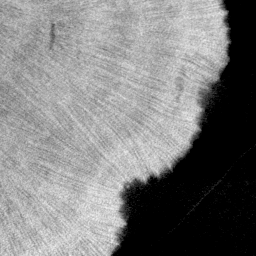
\includegraphics[width=1\textwidth, valign=c]{images/label-example-1.png}
    \end{subfigure}
    ~
    \begin{subfigure}[t]{0.32\textwidth}
        \centering
        
\includegraphics[width=1\textwidth, valign=c]{images/label-example-2.png}
    \end{subfigure}
    ~
    \begin{subfigure}[t]{0.32\textwidth}
        \centering
        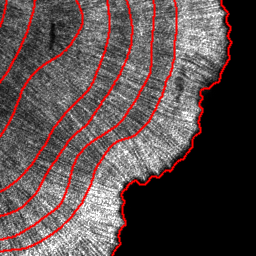
\includegraphics[width=1\textwidth, valign=c]{images/label-example-3.png}
    \end{subfigure}
    \caption{An example of a manually labelled 2D slice from the dataset used in this project. This represents the ideal semantic segmentation of a slice. \textbf{(left)} An unaltered section of a 2D slice taken from a 3D scan of a coral sample. The slice is a negative; brighter pixels correspond to high density and darker pixels correspond to low density. \textbf{(centre)} The manual labelling of the section. The white pixels correspond to the ``part of a boundary'' class, and the black pixels correspond to the ``not part of a bounary'' class. \textbf{(right)} The manual labelling overlaid with the corresponding section of the slice. The contrast and brightness of the slice has been altered to better show the annual banding, and the colour of the labelling has been changed for illustration purposes.}
    \label{fig:example-label}
\end{figure}

Several forms of deep convolutional neural networks (CNNs) currently achieve the state-of-the-art in semantic segmentation\footnote{\url{https://paperswithcode.com/task/semantic-segmentation/latest}}~\cite{chen2018encoder, semanticseg-SOTA}. For this project, pre-existing CNN architectures used for semantic segmentation that perform well on existing datasets are a reasonable starting point. Several CNN architectures will be repurposed and/or modified to process the skeletal density data.

The main architecture experimented with will be the U-Net architecture~\cite{ronneberger2015u}. U-Net was initially used to perform semantic segmentation on biomedical images such as images of cells on glass that were recorded with differential interference contrast microscopy. The U-Net architecture has not yet been applied to coral density data and experimentation with the U-Net architecture and the dataset used in this project could yield interesting results. To the best of the author's knowledge, none of the architectures experimented with throughout this project have ever been applied to coral skeleton density data of any kind. This project aims to not only determine how well multiple architectures perform in segmenting the skeletal density data but also to determine if CNNs are currently a viable solution to this task.

\section{Challenges}
\label{sec:challenges}

There are multiple challenges involved in the implementation of an automated solution. This section outlines and briefly discusses the most significant of these challenges.

\subsection{Labelling}

As previously discussed, the process of manually labelling the boundaries present in the data is time consuming. Labelling enough data for a CNN to perform well would require tens of hours of work. This process takes particularly long as appropriate slices must be extracted from the 3D CT data using a 3D visualisation program such as Avizo\footnote{\url{https://tiny.cc/avizo}} before they can be labelled. Not only is this process time consuming, it is also challenging. This is especially the case for a person who has not dealt with coral skeleton density data before. Before samples can be manually labelled, an acceptable standard of labelling must be approved by an expert.

\subsection{Class imbalance}

Another challenge involved with this project is dealing with the inherent class imbalance of the boundary labels. In a typical classification problem, class imbalance occurs when one class contains significantly fewer samples than the other classes. Since semantic segmentation can be seen as per-pixel classification, class imbalance can be an issue in this task as well. Looking at Figure \ref{fig:example-label}, it can be seen that the ratio of white to black pixels in the label is significantly low; there is a severe class imbalance between the ``part of a boundary'' and ``not part of a boundary'' classes. When a class imbalance exists within training data, supervised learning models will typically over-classify the ``majority'' groups due to their increased prior probabilities. As a result, the instances belonging to ``minority'' groups are misclassified more often than those belonging to the majority groups~\cite{classimbalance}.

This class imbalance gives rise to another challenge when assessing the performance of a model in its segmentation of the density data. Since the boundary labels are only one pixel wide, a model that predicts boundary positions that are just one pixel off of the correct positions could potentially achieve a standard per-pixel accuracy of 0\%. To solve this problem, a custom accuracy metric must be conceived, which rewards a model even when it predicts a boundary a few pixels away from the manually labelled position.

\subsection{Loading Three Dimensional Data}

When implementing an architecture capable of segmenting data in three dimensions, existing deep learning libraries---such as the Keras\footnote{\url{https://keras.io}} library used throughout this project---make the implementation of a 3D architecture relatively straightforward. However, as of the time of writing, a 3D ``data loader'' capable of loading 3D data from a directory and performing online data augmentation does not yet exist for the Keras library and would have to be designed and implemented.

\section{Related Work}

Although many examples of coral species classification using deep learning exist, no machine learning techniques of any kind have been applied to CT scans of coral skeletons. The implementation of an automated system capable of extracting the density banding or calculating the linear extension and calcification rates has not yet been attempted or at least published.

Steffens et al.~\cite{steff} make use of the DeeplabV3~\cite{deeplab} CNN to segment coral reef images into different types of substrates. However, the ImageCLEFcoral\footnote{\url{https://www.imageclef.org/2019/coral}} dataset that they use to test their implementation consists of images taken of the surfaces of coral reefs. Alonso et al.~\cite{alonso} segment coral reef images of a similar kind from the Eilat Fluorescence Corals dataset~\cite{eilat} using the SegNet CNN architecture~\cite{segnet}. Again, this work attempts to segment images taken of the surfaces of coral reefs rather than any kind of data representing the internals of a coral skeleton.

Three dimensional implementations of the U-Net architecture do exist. For example, {\c{C}}i{\c{c}}ek et al.~\cite{cicek} modify the U-Net architecture to process 3D data by replacing all 2D operations with their 3D counterparts. They assess the performance of their model on a dataset of Xenopus kidney embryos and propose both semi-automated and fully-automated use cases of the model. It is worth noting that the segmentation task that they attempt does not give rise to a class imbalance, and the nature of the segmentation that this project attempts is dissimilar due to the sparsity of the coral density band boundaries.

% {\bf A compulsory chapter,     of roughly $5$ pages}
% \vspace{1cm} 

% \noindent
% This chapter should describe the project context, and motivate each of
% the proposed aims and objectives.  Ideally, it is written at a fairly 
% high-level, and easily understood by a reader who is technically 
% competent but not an expert in the topic itself.

% In short, the goal is to answer three questions for the reader.  First, 
% what is the project topic, or problem being investigated?  Second, why 
% is the topic important, or rather why should the reader care about it?  
% For example, why there is a need for this project (e.g., lack of similar 
% software or deficiency in existing software), who will benefit from the 
% project and in what way (e.g., end-users, or software developers) what 
% work does the project build on and why is the selected approach either
% important and/or interesting (e.g., fills a gap in literature, applies
% results from another field to a new problem).  Finally, what are the 
% central challenges involved and why are they significant? 
 
% The chapter should conclude with a concise bullet point list that 
% summarises the aims and objectives.  For example:

% \begin{quote}
% \noindent
% The high-level objective of this project is to reduce the performance 
% gap between hardware and software implementations of modular arithmetic.  
% More specifically, the concrete aims are:

% \begin{enumerate}
% \item Research and survey literature on public-key cryptography and
%       identify the state of the art in exponentiation algorithms.
% \item Improve the state of the art algorithm so that it can be used
%       in an effective and flexible way on constrained devices.
% \item Implement a framework for describing exponentiation algorithms
%       and populate it with suitable examples from the literature on 
%       an ARM7 platform.
% \item Use the framework to perform a study of algorithm performance
%       in terms of time and space, and show the proposed improvements
%       are worthwhile.
% \end{enumerate}
% \end{quote}

\section{Summary of Objectives}

In summary, the main objective of this project is to automate the estimation of the calcification rate---the amount of skeletal matter produced annually by corals. This objective is broken down into multiple tasks:

\begin{enumerate}
    \item Curate a dataset of image-label pairs from the initial unlabelled dataset provided.
    \item Train existing two dimensional convolutional neural network architectures to extract the annual density boundaries present in the data.
    \item Modify the architectures to process three dimensional data.
    \item Conceive and implement an accuracy metric to assess the performance of different networks on the data.
    \item Optimise hyperparameters of the chosen network architecture to maximise accuracy.
    \item Perform ablation studies to gain a better understanding of the architectures used.
    \item Make use of these extracted boundaries to automate the calculation of the annual skeletal matter produced.
    \item Package the implementation in a form usable by researchers at the Natural History Museum and the School of Earth Sciences at the University of Bristol.
\end{enumerate}


\chapter{Technical Background}
\label{chap:technical}
% {\bf A compulsory chapter,     of roughly $10$ pages} 
% \vspace{1cm} 

% \noindent
% This chapter is intended to describe the technical basis on which execution
% of the project depends.  The goal is to provide a detailed explanation of
% the specific problem at hand, and existing work that is relevant (e.g., an
% existing algorithm that you use, alternative solutions proposed, supporting
% technologies).  

% Per the same advice in the handbook, note there is a subtly difference from
% this and a full-blown literature review (or survey).  The latter might try
% to capture and organise (e.g., categorise somehow) {\em all} related work,
% potentially offering meta-analysis, whereas here the goal is simple to
% ensure the dissertation is self-contained.  Put another way, after reading 
% this chapter a non-expert reader should have obtained enough background to 
% understand what {\em you} have done (by reading subsequent sections), then 
% accurately assess your work.  You might view an additional goal as giving 
% the reader confidence that you are able to absorb, understand and clearly 
% communicate highly technical material.

As outlined in Chapter \ref{chap:context}, the objective of this project is to use deep learning to automate the calculation of the amount of skeletal matter produced by corals annually. This chapter introduces and briefly describes the techniques used in order to achieve this goal.

\section{Deep Learning}
\label{sec:deeplearning}

Based loosely on the structure of the brain, artificial neural networks (ANNs) are computational models that have proved useful in a wide range of applications~\cite{lecun2015deep, healthcare, nlp}\textemdash a notable example being the recent success of convolutional neural networks in the field of computer vision~\cite{compvision, semanticsegreview}. Deep learning is a form of machine learning that concerns the use of ANNs with many layers\textemdash hence the name ``deep'' learning. The field has seen a significant increase in popularity in recent years since a network named AlexNet famously won the ImageNet Large Scale Visual Recognition Challenge in 2012\footnote{\url{http://www.image-net.org/challenges/LSVRC/2012/results.html}}, performing considerably better than the previous state-of-the-art~\cite{alexnet}.

A typical fully connected ANN is a layered network of ``neurons'' connected by a series of ``weights''. A neuron is simply an object that produces a weighted sum of some number of inputs. This weighted sum is often passed through a non-linear ``activation'' function and the final result is referred to as the ``activation'' of the neuron. When values are supplied to the input neurons of the network, these values are forward-propagated through the network, activating each layer of neurons which, in turn, activate the next layer. The resulting activations of the neurons in the final layer are the output of the network.

\subsection{Convolutional Neural Networks}

The convolutional neural network (CNN) is a type of neural network named after the discrete convolution operation that sets these models apart from typical fully connected ANNs. The convolution operation makes use of surrounding pixels in order to change the value of a central pixel. The 2D discrete convolution operation is defined as

\begin{equation}
    g(x,y)=\sum_{i=1}^{m}\sum_{j=1}^{n}f(x-j,y-k)h(j,k)
\end{equation}

\noindent
where $f$ is the input image, $h$ is an $m\times n$ kernel, and $g$ is the resulting image.

CNNs often contain multiple convolutional layers in which increasingly complex features of an image may be detected by making use of a combination of simpler features detected in previous layers. A convolutional layer convolves the channels of an image with multiple learned kernels. A channel is simply a component of an image\textemdash an RGB image, for example, consists of three channels, whilst a greyscale image consists of only one. The output of these operations will be multiple modified images that are referred to as ``feature maps''. These feature maps can then be used as the input channels to the next layer, and so on.

As well as the convolution operation, the max-pooling operation is often used. The max-pooling operation is used to decrease the dimensionality of the input in attempt to force the network to ``learn'' features present in the input. These operations are illustrated in Figure \ref{fig:operations}.

\begin{figure}[t]
    \centering
    \begin{subfigure}[t]{0.43\textwidth}
        \centering
        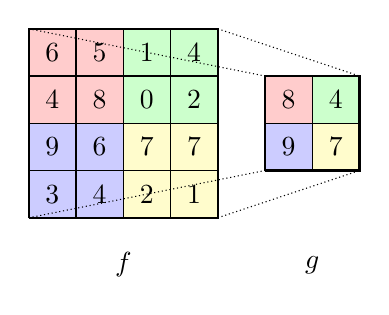
\begin{tikzpicture}[scale=0.6]
    \filldraw[color=blue, opacity=0.2] (0,0) rectangle (2,2);
    \filldraw[color=red, opacity=0.2] (0,2) rectangle (2,4);
    \filldraw[color=green, opacity=0.2] (2,2) rectangle (4,4);
    \filldraw[color=yellow, opacity=0.2] (2,0) rectangle (4,2);

    \filldraw[color=blue, opacity=0.2] (5,1) rectangle (6,2);
    \filldraw[color=red, opacity=0.2] (5,2) rectangle (6,3);
    \filldraw[color=green, opacity=0.2] (6,2) rectangle (7,3);
    \filldraw[color=yellow, opacity=0.2] (6,1) rectangle (7,2);

	\draw [thick] (0,0) -- (0,4) -- (4,4) -- (4,0) -- (0,0);
    \draw (0,1) -- (4,1);
    \draw (0,2) -- (4,2);
    \draw (0,3) -- (4,3);
    \draw (1,0) -- (1,4);
    \draw (2,0) -- (2,4);
    \draw (3,0) -- (3,4);
    \node at (0.5, 0.5) {3};
    \node at (1.5, 0.5) {4};
    \node at (2.5, 0.5) {2};
    \node at (3.5, 0.5) {1};
    \node at (0.5, 1.5) {9};
    \node at (1.5, 1.5) {6};
    \node at (2.5, 1.5) {7};
    \node at (3.5, 1.5) {7};
    \node at (0.5, 2.5) {4};
    \node at (1.5, 2.5) {8};
    \node at (2.5, 2.5) {0};
    \node at (3.5, 2.5) {2};
    \node at (0.5, 3.5) {6};
    \node at (1.5, 3.5) {5};
    \node at (2.5, 3.5) {1};
    \node at (3.5, 3.5) {4};
    
    \draw[densely dotted] (0,0) -- (5,1);
    \draw[densely dotted] (0,4) -- (5,3);
    \draw[densely dotted] (4,4) -- (7,3);
    \draw[densely dotted] (4,0) -- (7,1);
    
    \draw [thick] (5,1) -- (5,3) -- (7,3) -- (7,1) -- (5,1);
    \draw (6,1) -- (6,3);
    \draw (5,2) -- (7,2);
    
    \node at (5.5, 1.5) {9};
    \node at (6.5, 1.5) {7};
    \node at (5.5, 2.5) {8};
    \node at (6.5, 2.5) {4};
    
    \node at (2, -1) {$f$};
    \node at (6, -1) {$g$};
\end{tikzpicture}
    \vspace*{1mm}
    \caption{2D Max-pooling}
    \end{subfigure}
    ~
    \begin{subfigure}[t]{0.55\textwidth}
        \centering
        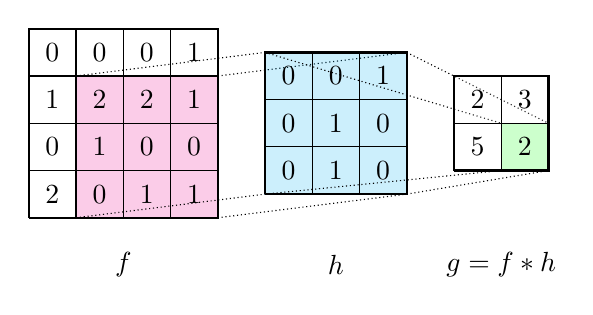
\begin{tikzpicture}[scale=0.6]
    \filldraw[color=magenta, opacity=0.2] (1,0) rectangle (4,3);

	\draw [thick] (0,0) -- (0,4) -- (4,4) -- (4,0) -- (0,0);
    \draw (0,1) -- (4,1);
    \draw (0,2) -- (4,2);
    \draw (0,3) -- (4,3);
    \draw (1,0) -- (1,4);
    \draw (2,0) -- (2,4);
    \draw (3,0) -- (3,4);
    
    \node at (0.5, 0.5) {2};
    \node at (1.5, 0.5) {0};
    \node at (2.5, 0.5) {1};
    \node at (3.5, 0.5) {1};
    \node at (0.5, 1.5) {0};
    \node at (1.5, 1.5) {1};
    \node at (2.5, 1.5) {0};
    \node at (3.5, 1.5) {0};
    \node at (0.5, 2.5) {1};
    \node at (1.5, 2.5) {2};
    \node at (2.5, 2.5) {2};
    \node at (3.5, 2.5) {1};
    \node at (0.5, 3.5) {0};
    \node at (1.5, 3.5) {0};
    \node at (2.5, 3.5) {0};
    \node at (3.5, 3.5) {1};
    
    \draw[densely dotted] (1,0) -- (5,0.5);
    \draw[densely dotted] (1,3) -- (5,3.5);
    \draw[densely dotted] (4,3) -- (8,3.5);
    \draw[densely dotted] (4,0) -- (8,0.5);
    
    \filldraw[color=cyan, opacity=0.2] (5,0.5) rectangle (8,3.5);
    
    \draw [thick] (5,0.5) -- (5,3.5) -- (8,3.5) -- (8,0.5) -- (5,0.5);
    \draw (5,2.5) -- (8,2.5);
    \draw (5,1.5) -- (8,1.5);
    \draw (6,0.5) -- (6,3.5);
    \draw (7,0.5) -- (7,3.5);
    
    \node at (5.5, 1) {0};
    \node at (6.5, 1) {1};
    \node at (7.5, 1) {0};
    \node at (5.5, 2) {0};
    \node at (6.5, 2) {1};
    \node at (7.5, 2) {0};
    \node at (5.5, 3) {0};
    \node at (6.5, 3) {0};
    \node at (7.5, 3) {1};
    
    \draw[densely dotted] (5,0.5) -- (10, 1);
    \draw[densely dotted] (5,3.5) -- (10, 2);
    \draw[densely dotted] (8,3.5) -- (11, 2);
    \draw[densely dotted] (8,0.5) -- (11, 1);
    
    \filldraw[color=white, opacity=0.2] (9,1) rectangle (10,2);
    \filldraw[color=white, opacity=0.2] (9,2) rectangle (10,3);
    \filldraw[color=green, opacity=0.2] (10,1) rectangle (11,2);
    \filldraw[color=white, opacity=0.2] (10,2) rectangle (11,3);
    
    \draw [thick] (9,1) -- (9,3) -- (11,3) -- (11,1) -- (9,1);
    \draw (10,1) -- (10,3);
    \draw (9,2) -- (11,2);
    
    \node at (9.5, 1.5) {5};
    \node at (10.5, 1.5) {2};
    \node at (9.5, 2.5) {2};
    \node at (10.5, 2.5) {3};
    
    \node at (2, -1) {$f$};
    \node at (6.5, -1) {$h$};
    \node at (10, -1) {$g=f\ast h$};
\end{tikzpicture}
        \vspace*{1mm}
        \caption{2D Convolution}
    \end{subfigure}
    \caption{Illustrations of the 2D max-pooling and convolution operations. \textbf{(a)} The max-pooling operation shown takes an input image $f$ and uses a 2$\times$2 filter and stride of two to produce the output image $g$. Note that the maximum value in each coloured region of the input is the resulting value of the corresponding regions of the output. \textbf{(b)} The convolution operation shown takes an input image $f$ and uses a 3$\times$3 kernel $h$ with a stride of one to produce the output image $g=f\ast h$, where $\ast$ denotes the convolution operation. Note that the kernel shown in the convolution operation is ``flipped'' in both the $x$ and $y$ axes before the element-wise multiplication and summation takes place.}
    \label{fig:operations}
\end{figure}

Another feature of CNNs that set them apart from their fully connected counterparts is the localised ``receptive fields'' of the neurons present in convolutional layers. Whilst neurons present in a fully connected layer can receive input from every neuron in the previous layer, neurons present in a convolutional layer can only receive input from a small amount of neighbouring neurons in the previous layer. For example, if a 3$\times$3 kernel is used, a neuron's activation can only be influenced by nine neurons in the previous layer. This area of input that can influence a neuron is called its receptive field. This is one of the reasons why during hyper parameter optimisation, kernel sizes from various layers may be tuned in order to increase or decrease the size of neurons' receptive fields. Hyper parameter optimisation is discussed in Section \ref{sec:hyperparam}.

\subsection{Backpropagation}
\label{sec:backprop}

First popularised by Rumelhart et al. in 1986~\cite{rumelhart}, the backpropagation algorithm is still the main learning mechanism used in neural networks today. Once a loss function is defined to measure the performance of the network, backpropagation can be used to compute the derivative of the loss function with respect to each weight in the network using the chain rule. The derivatives are calculated one layer at a time, iterating backward from the output layer. Since the backpropagation algorithm makes use of the chain rule, the loss function must be differentiable. This must also be the case for the chosen activation functions for each neuron.

An optimisation algorithm can then use these computed derivatives to adjust each weight in order to minimise the chosen loss function. Loss functions used throughout this project are discussed in Section \ref{sec:loss}.

\subsection{Optimisation Algorithms}

Once the derivatives\textemdash or ``gradients''\textemdash have been calculated, an optimisation algorithm is used to determine the exact value each weight should be updated to. When training deep neural networks, some variant of the gradient descent algorithm is often used. Gradient descent~\cite[p. 536]{gradient} is an iterative algorithm designed to find local minima of some differentiable function\textemdash in this case, the loss function. A visualisation of the gradient descent algorithm is shown in Figure \ref{fig:gd}. The gradient descent algorithm evaluates the loss function over the entire dataset before taking a ``step'' in the direction of the gradient computed. A step consists of updating the value of every weight in order to decrease the average loss value that would be achieved by the network when processing the dataset. Evaluating the loss function over the entire dataset once is referred to as an ``epoch''.

The size of the weight update is not only determined by the gradient calculated, but also by a hyper parameter called the ``learning rate''. For example, gradient descent calculates the update for a single weight $w$ as

\begin{equation}
    w := w - \eta\nabla\ell(w)
\end{equation}

\noindent
where $\eta$ is the learning rate and $\nabla\ell(w)$ is the derivative of the loss function $\ell$ with respect to $w$. Choosing an appropriate learning rate is challenging but is essential to allow an optimisation algorithm to converge to a local minimum. A learning rate that is too large can cause the loss function to fluctuate around the minimum, impeding convergence or even causing divergence. The learning rate hyper parameter has a significant effect on training and is one of the most important parameters tuned in the hyper parameter optimisation process (see Section \ref{sec:hyperparam}).


\subsubsection{Stochastic Gradient Descent}

Issues arise when using gradient descent with larger datasets, as evaluating the loss function over the entire dataset before a step can be taken becomes increasingly computationally costly~\cite{gdbad}. These issues have given rise to the popularity of the stochastic gradient descent (SGD) and the mini-batch gradient descent optimisation algorithms. SGD is a variant of the gradient descent algorithm that takes a step each time a sample is processed rather than only once the entire dataset is processed. Mini-batch gradient descent is yet another variant of gradient descent in which weights are updated after evaluating the loss function over a subset\textemdash or ``batch''\textemdash of the training samples.

\begin{figure}[t]
    \centering
    \begin{tikzpicture}[scale=1.1]
	\begin{axis}[
% 	colormap/greenyellow,
	colormap name=cool2,
% 	view={0}{90}
	xlabel=$x$,
	ylabel=$y$,
	zlabel=Loss,
	zmin=0.1, zmax=1.9,
	xtick distance=175,
	ytick distance=175,
	xticklabels=\empty,
	yticklabels=\empty,
	zticklabels=\empty
	]
% 	\addplot3[surf,
% 		domain=0:360,samples=40] 
% 		{0.5*sin(x-100)*sin(y-50) - 0.000005*((x-100)^2) + 0.000005*((y-50)^2) + 1};
    \addplot3 [surf, mesh/rows=36] table [x=xs, y=ys, z=zs, col sep=comma] {csv/surf.csv};
    
	\addplot3 [black, mark=*, line width=0.8pt, mark size=0.8pt] table [x=xs, y=ys, z=zs, col sep=comma] {csv/sgd.csv};
	
	\addplot3 [black, mark=*, line width=0.8pt, mark size=0.8pt] table [x=xs, y=ys, z=zs, col sep=comma] {csv/sgd3.csv};
	
	\node[] at (axis cs: 320, 200, 1.9) {\scriptsize{($x_0, y_0, \ell(x_0, y_0)$)}};
	
	\node[] at (axis cs: 260, 200, 0.1) {\scriptsize{($x_n, y_n, \ell(x_n, y_n)$)}};
	\end{axis}
\end{tikzpicture}
    \caption{A diagram visualising the gradient descent algorithm for a model containing two trainable parameters, $x$ and $y$. Given a random starting configuration with parameters $x_0$ and $y_0$, the average loss value that would be achieved when processing the entire dataset is given by $\ell(x_0, y_0)$. Say gradient descent takes $n$ steps in the direction of steepest descent at each iteration until the loss value converges to some local minimum, $x_n$ and $y_n$ would be the final parameter values and the final loss would be $\ell(x_n, y_n)$. It is worth noting that even though the two starting configurations shown in the diagram both converge to the same local minimum, this might not always be the case. A starting configuration nearer to one of the other possible local minima would most likely not converge to the example local minimum $\ell(x_n, y_n)$ shown.}
    \label{fig:gd}
\end{figure}

\subsubsection{Adam}

First introduced by Kingma and Ba in 2014, Adam~\cite{adam} is an optimisation algorithm that is also based off of SGD. However, rather than using the same learning rate across all parameters, Adam computes individual adaptive learning rates for different parameters. These individual learning rates are based off of estimates of the first moment (the mean) and second moment (the uncentered variance) of the gradients~\cite{gdbad}. Kingma and Ba showed empirically that Adam works well in practice and compares favourably to other optimisation algorithms when optimising both fully connected ANNs and deep CNNs.

\subsection{Loss functions}
\label{sec:loss}

A loss function takes both the actual and predicted values of a training sample, and outputs some measure of how well a model performed by producing that prediction. As mentioned in Section \ref{sec:backprop}, backpropagation makes use of the derivative of the loss function with respect to each parameter in order to minimise the loss achieved. If the appropriate loss function is chosen, minimising the loss should improve the performance achieved by the network. It is for this reason that loss functions must be differentiable. The loss functions that were experimented with throughout this project are outlined below.

\subsubsection{Binary Cross-Entropy Loss}

The binary cross-entropy loss function is used when classifying samples that can belong to two classes. When performing image classification, a model will produce two probabilities\textemdash one for each class. When performing image segmentation, a model effectively classifies each pixel; thus, two probabilities will be produced for each pixel. These are the model's predicted probabilities that a given image (or pixel) belongs to each of the two classes. Since these two classes are the only possible classes that the model can predict, the probabilities should sum to one. The binary cross-entropy loss is defined as:

\begin{equation}
    CE(p, y) = 
    \begin{cases}
        -\log(p) & \text{if } y = 1\\
        -\log(1 - p) & \text{otherwise}
    \end{cases}
\end{equation}

where $y \in \{+1, -1\}$ is the actual value (the ground-truth), and $p \in [0, 1]$ is the model's estimated probability for the class with label $y = 1$. This is the loss value achieved when classifying a single training sample.

\subsubsection{Binary Focal Loss}

\begin{figure}[t]
    \centering
    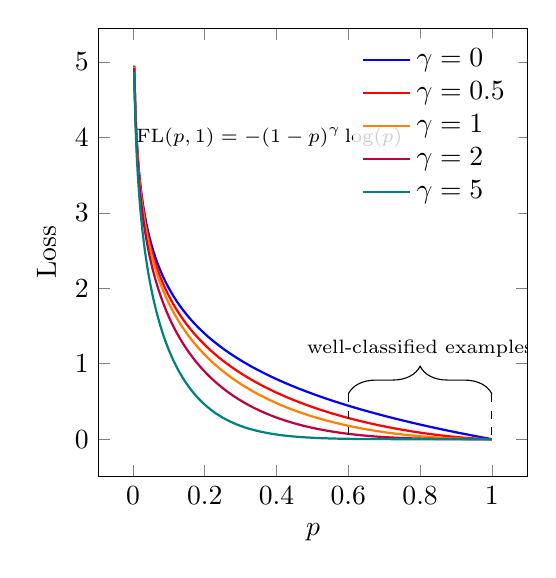
\begin{tikzpicture}
	\begin{axis}[
		xlabel=$p$,
		ylabel=Loss,
		width=0.58\textwidth,
        height=\axisdefaultheight,
        legend cell align=left,
        legend style={fill=white, fill opacity=0.8, draw=none,text opacity=1}
	]
	
	\addplot[samples=300, domain=0:1, thick, blue]   {2 * -(1-x)^0   * log10(x)};
	\addlegendentry{$\gamma = 0$}
	\addplot[samples=300, domain=0:1, thick, red]    {2 * -(1-x)^0.5 * log10(x)};
	\addlegendentry{$\gamma = 0.5$}
	\addplot[samples=300, domain=0:1, thick, orange] {2 * -(1-x)^1   * log10(x)};
	\addlegendentry{$\gamma = 1$}
	\addplot[samples=300, domain=0:1, thick, purple] {2 * -(1-x)^2   * log10(x)};
	\addlegendentry{$\gamma = 2$}
	\addplot[samples=300, domain=0:1, thick, teal]   {2 * -(1-x)^5   * log10(x)};
	\addlegendentry{$\gamma = 5$}
	
	\node[] at (0.38, 4) {\scriptsize{$\text{FL}(p, 1) = -(1 - p)^{\gamma} \log (p)$}};
	\draw [decorate,decoration={brace,amplitude=10pt}]
	(0.6, 0.6) -- (1, 0.6) node[midway]{};
	\node[] at (0.8, 1.2) {\scriptsize{well-classified examples}};
	\draw[dashed] (0.6, 0.6) -- (0.6, 0);
	\draw[dashed] (1, 0.6) -- (1, 0);
	\end{axis}
\end{tikzpicture}
    \caption{An illustration of the focal loss with varying values of $\gamma$. Recreated from \cite{focalloss}: ``setting $\gamma > 0$ reduces the relative loss for well-classified examples $(p > 0.5)$, putting more focus on hard, misclassified examples''.}
    \label{fig:focal}
\end{figure}

Proposed by Lin et al. in 2018, the Focal Loss~\cite{focalloss} is designed to address the ``class imbalance'' problem. In a typical classification problem, class imbalance occurs when one class contains significantly fewer samples than the other classes. Lin et al. highlight the fact that when using the cross-entropy loss function, even samples that are well-classified incur a loss with ``non-trivial'' magnitude. When summed over large numbers of samples from the easily classified majority class, these small loss values can overwhelm the loss resulting from the minority class samples~\cite{focalloss}.

In an attempt to address this problem, the focal loss introduces two new parameters: a weighting factor $\alpha \in [0, 1]$ and a ``focusing'' parameter $\gamma \geq 0$.
The binary focal loss is then defined as:

\begin{equation}
    \text{FL}(p, y) = 
    \begin{cases}
        -\alpha(1 - p)^{\gamma} \log (p) & \text{if } y = 1\\
        (1 - \alpha)p^{\gamma} \log (1 - p) & \text{otherwise}
    \end{cases}
\end{equation}

where $y \in \{+1, -1\}$ is the actual value (the ground-truth), and $p \in [0, 1]$ is the model's estimated probability for the class with label $y = 1$. The weighting factor increases the loss produced by the misclassification of minority class samples whilst the focusing factor ``reduces the contribution from easy examples and extends the range in which an example receives low loss''~\cite{focalloss}. When $\gamma = 0$ and $\alpha = 1$, the focal loss is equivalent to the cross-entropy loss. The contribution of the $\gamma$ value to the loss produced can be seen in Figure \ref{fig:focal}.

\subsection{Accuracy Metrics}

Although loss functions can be used to measure performance, their main purpose is to be used to train the network. To quantify the performance achieved by a network, an accuracy metric should instead be used. Accuracy metrics do not play a direct role in training networks, though they can be used indirectly\textemdash for example, to determine whether or not to continue training. Choosing an appropriate accuracy metric is essential and proved challenging throughout this project. The main accuracy metric decided upon was based off of the Hausdorff distance discussed in Section \ref{sec:hausdorff}.

\subsection{Overfitting}

The term overfitting is used to describe when a model performs well on the data on which it is trained, yet poorly on data which it has not yet been exposed to. Due to the nature of deep learning systems?? overfitting is a significatn problem? something cite. Many techniques can be utilised in order to minimize overfitting.

\subsubsection{Data augmentation}

A very common technique used to reduce overfitting is data augmentation. Data augmentation is the process of augmenting the labelled training data in some way in order to increase the amount of training data available. This augmentation can be performed ``online'' with each training sample being randomly augmented during the training process, or it can be performed ``offline'' with the augmentation taking place before training. The training data can be augmented in many ways. Common examples for 2D images are: random rotations within some predefined range, random changes to brightness levels, and random horizontal and vertical flips. Explain here why or how data augmentation reduces overfitting?

\subsubsection{Dropout}

Another technique often used to reduce overfitting is ``dropout''. When was dropout introduced? is it used in any really famous successful papers or networks? Explain what dropout is. Explain how it is used to reduce overfitting.

\subsubsection{Cross-Validation}

Introduce train test val split and what they are all used for.

\subsubsection{Early Stopping}
Referred to as a ``beautiful free lunch'' by Geoffrey Hinton~\cite[p. 141]{earlystopping}, early stopping is.

\subsection{Ablation Studies}

\subsection{Hyper parameter optimisation}
\label{sec:hyperparam}

Define what a parameter and hyper parameter is. Talk about diff algorithms (genetic vs brute force).

\section{Network Architectures}

Various CNN architectures are experimented with throughout this project. This section introduces and details these architectures.

\subsection{SegNet}

In 2015, Badrinarayanan, Kendall, and Cipolla~\cite{segnet} introduced SegNet: a fully convolutional neural network architecture for semantic pixel-wise segmentation that was primarily motivated by road scene understanding applications. An architecture is ``fully convolutional'' when it contains no fully connected layers. The architecture consists of an ``encoder'' and a ``decoder'' with some pass through of information from layers early in the encoder to layers later in the decoder.

An encoder is a model or part of a model that takes some input and ``encodes'' the input into some lower dimensional representation. For example, a typical CNN architecture used for image classification is an example of an encoder since the input could be some high resolution two dimensional image and the output would be a small number of probabilities\textemdash one for each possible class that the image could be classified as. In fact, the encoder architecture used in SegNet is topologically identical to the convolutional layers used in the VGG16 architecture used for image classification~\cite{segnet, vgg16}. A decoder can be thought of as the opposite of an encoder; given some input, a decoder will ``decode'' the input back into some higher dimensional representation.

The decoder uses pooling indices computed in the max-pooling step of corresponding encoder layers to perform non-linear upsampling.

This eliminates the need for learning to upsample.

\subsection{U-Net}

Presented by Ronneberger et al. in 2015~\cite{ronneberger2015u}, U-Net is a convolutional neural network architecture that was initially used to perform image segmentation on biomedical images, but has since been used on a wider range of visual data. At a high level, the U-Net architecture consists of three sections: the contracting path, the bottleneck, and the expanding path. The contracting path follows the typical architecture of a convolutional network, in that the image is gradually downsampled via convolutional and max-pooling layers and the number of feature channels is increased. The expansion path then gradually reconstructs the image via `up-convolutions'. Throughout the expansion path, the feature channels from the corresponding contraction layers are appended to the feature channels in the expansion layers. This allows the features that are learned whilst contracting the image to also be used to reconstruct it. A diagram of the U-Net architecture is shown in Figure~\ref{fig:unet}.

The U-Net and SegNet architectures share multiple similarities. They are both fully convolutional architectures designed to perform semantic pixel-wise segmentation. Both architectures also consist of an encoder, a bottleneck, and a decoder, with the encoder following a typical CNN architecture. Note that when describing the U-Net architecture, Ronneberger et al. refer to the encoder and decoder as the contracting and expanding paths respectively. Another similarity between the architectures is their passing of information from layers in the encoder to corresponding layers in the decoder. However, the passing of information is implemented differently in each architecture. Whilst U-Net passes information by concatenating feature maps from layers in the encoder to the feature maps of layers in the decoder, SegNet passes information by ... 

\begin{figure}[t]
    \centering
    \begin{tikzpicture}[scale=0.4]
    \node[above] at (13, 3) {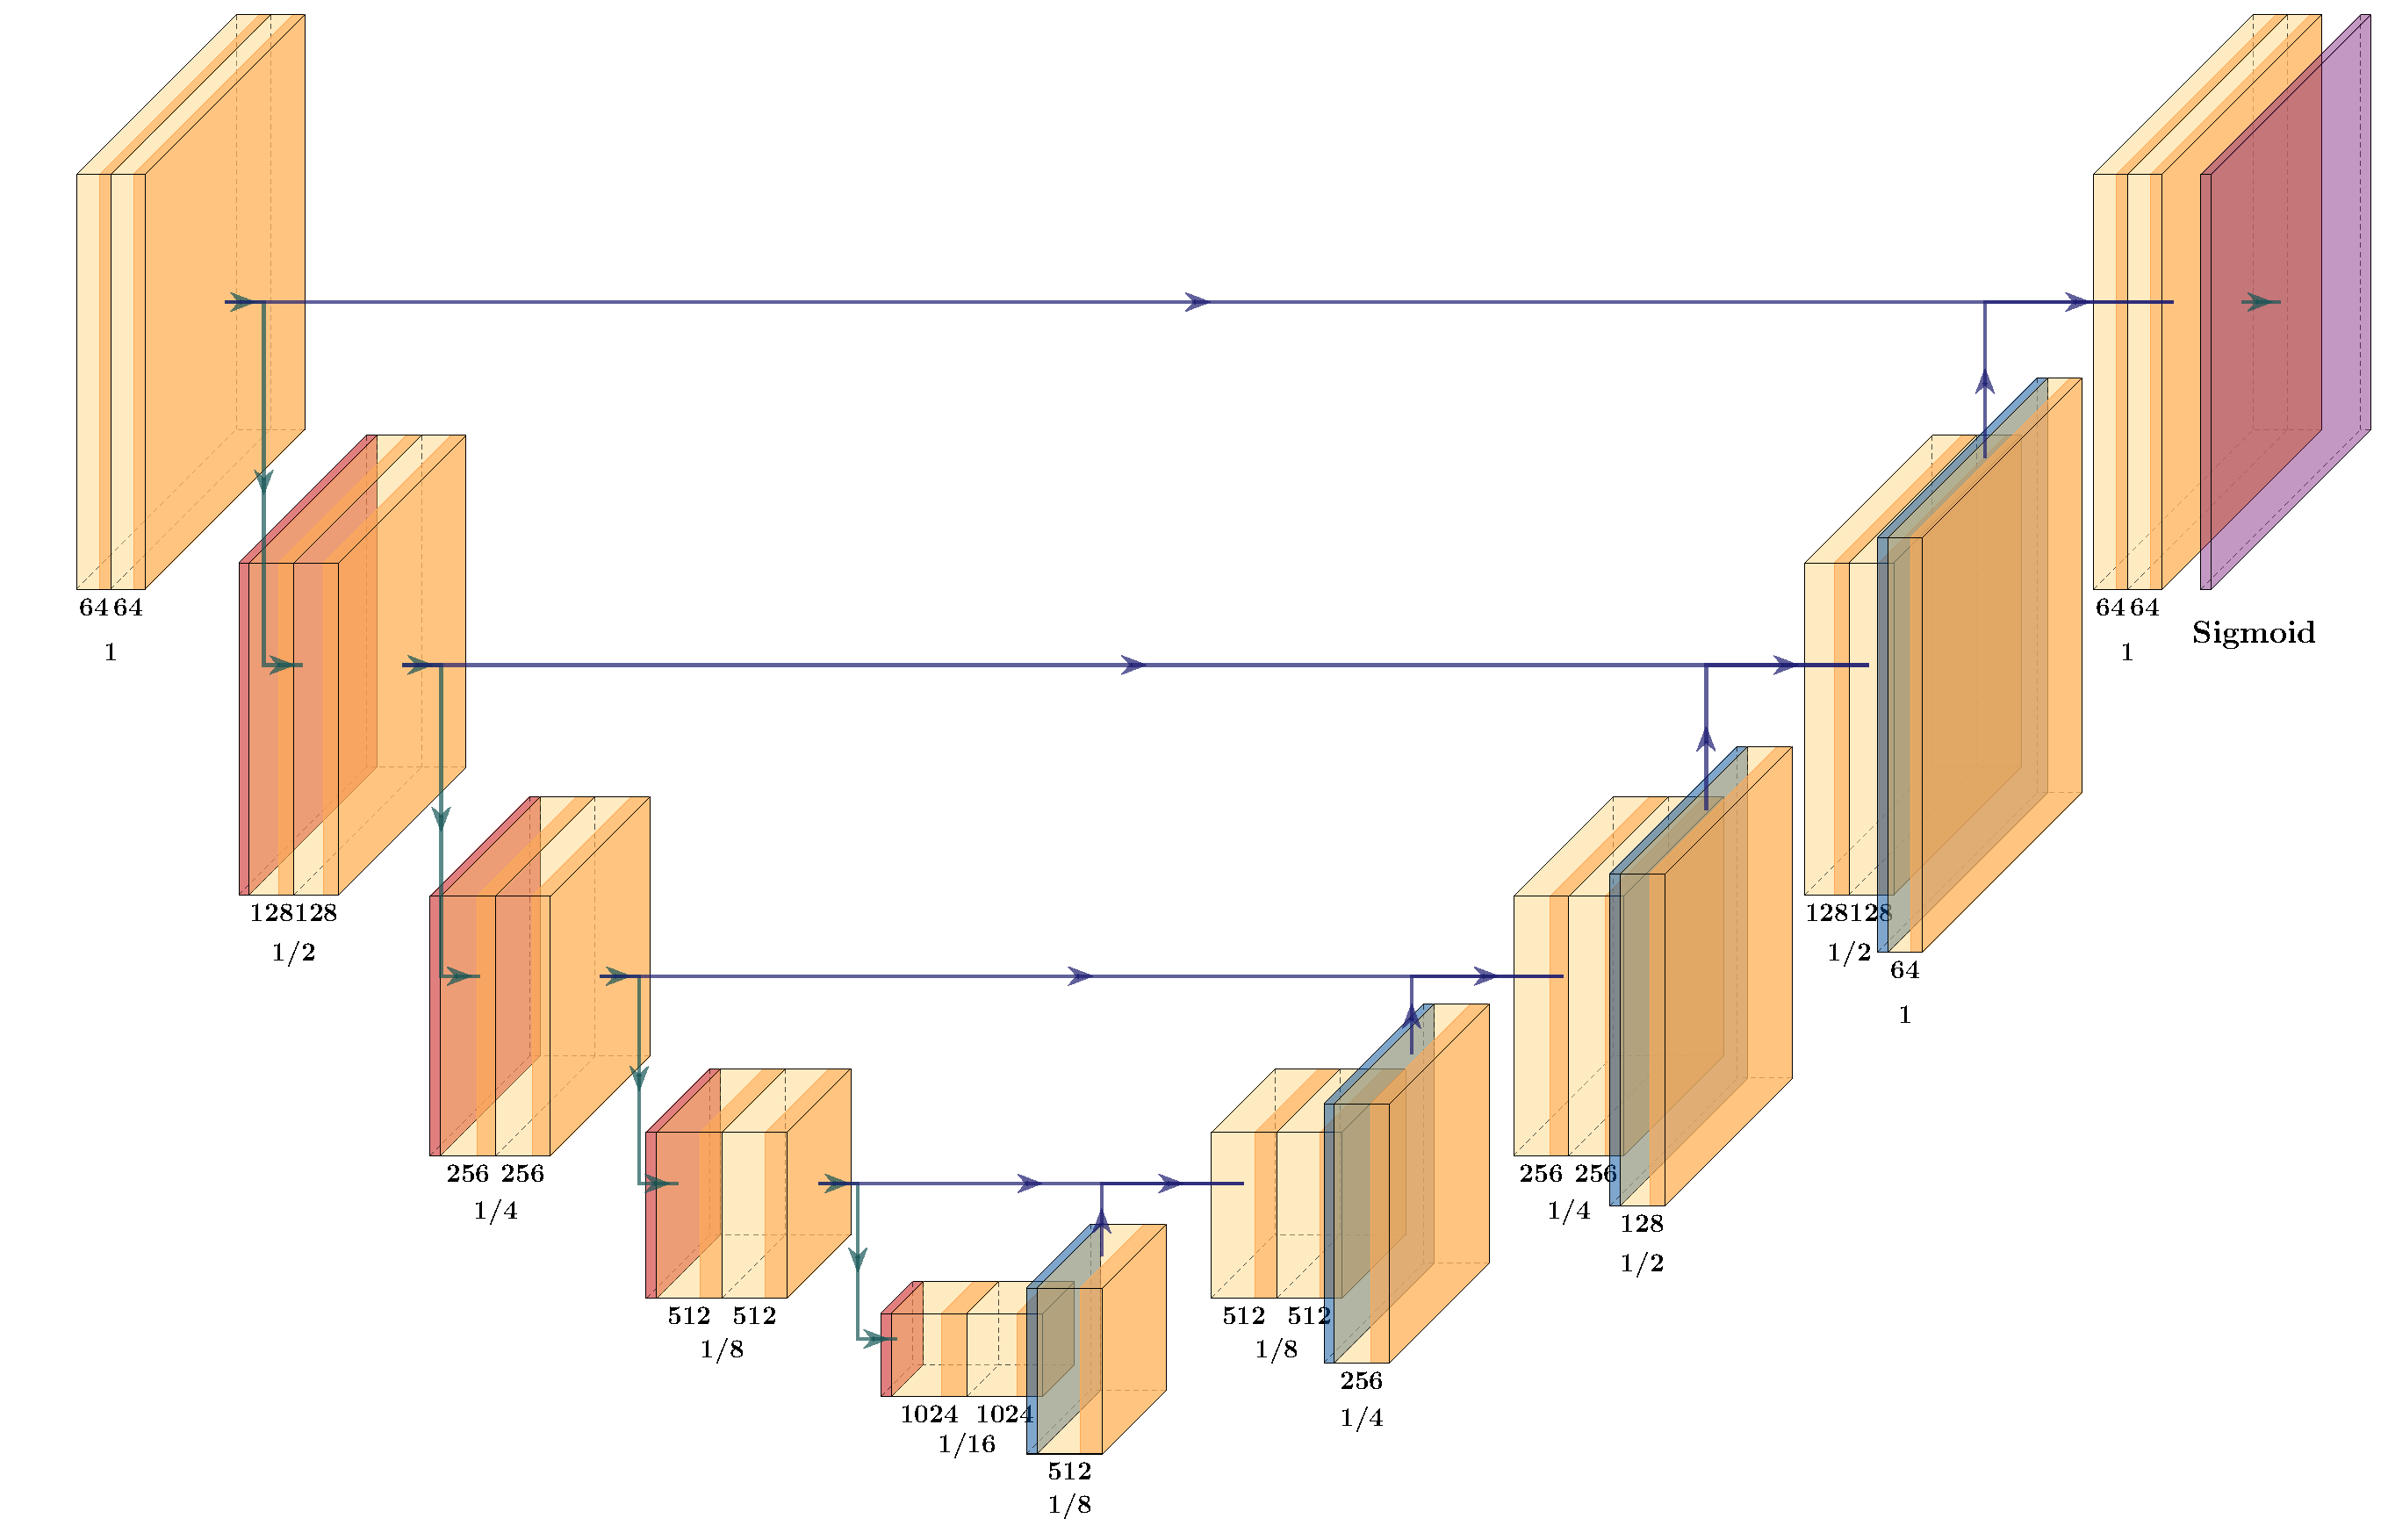
\includegraphics[width=1\textwidth]{images/U-Net.pdf}};
    
    \filldraw[color=\ConvColor, opacity=0.5] (0,1.5) rectangle (1,2.5);
    \draw[] (0,1.5) rectangle (1,2.5);
    \node[right] at (1, 2) {\scriptsize{3$\times$3 Convolution}};
    
    \filldraw[color=\ConvReluColor, opacity=0.8] (0,0) rectangle (1,1);
    \draw[] (0,0) rectangle (1,1);
    \node[right] at (1, 0.5) {\scriptsize{ReLU}};
    
    \filldraw[color=\PoolColor, opacity=0.75] (9,0) rectangle (10,1);
    \draw[] (9,0) rectangle (10,1);
    \node[right] at (10, 0.5) {\scriptsize{2$\times$2 Max-pooling}};
    
    \filldraw[color=\UnpoolColor, opacity=0.7] (9,1.5) rectangle (10,2.5);
    \draw[] (9,1.5) rectangle (10,2.5);
    \node[right] at (10, 2) {\scriptsize{2$\times$2 Up-convolution}};
    
    % \filldraw[color=\PoolColor, opacity=1] (18,0) rectangle (19,1);
    % \draw[] (18,0) rectangle (19,1);
    \node[right] at (19, 0.5) {\scriptsize{Feedforward}};
    
    % \filldraw[color=\PoolColor, opacity=1] (18,1.5) rectangle (19,2.5);
    % \draw[] (18,1.5) rectangle (19,2.5);
    \node[right] at (19, 2) {\scriptsize{Concatenation}};

    \begin{scope}[decoration={
        markings, mark=at position 0.75 with {\arrow[scale=1.5]{stealth}}}] 
        \draw[postaction={decorate}, color={rgb:blue,4;red,1;green,4;black,3}] (18,0.5)--(19,0.5);
        \draw[postaction={decorate}, color={rgb:blue,4;red,1;green,1;black,3}] (18,2)--(19,2);
    \end{scope}
\end{tikzpicture}
    \caption{A diagram of the U-Net architecture. Each cube represents a layer with the number of output feature maps shown at the bottom of the cube. At the bottleneck there are 1024 feature maps that are each one sixteenth the size of the input image in the $x$ and $y$ dimensions. The green arrows represent the feedforward of information from one layer to the next, whereas the blue arrows represent the concatenation of the feature maps of one layer to another.}
    \label{fig:unet}
\end{figure}

\subsection{CycleGANs and pix2pix}

Throughout this project, various deep learning techniques are utilised in an attempt to maximise the performance achieved.

\section{Classical Image Processing Techniques}

\subsection{Hausdorff distance}
\label{sec:hausdorff}

\section{Supporting Technologies}

\subsection{Keras}

The Keras\footnote{\url{https://keras.io}} library is used to implement all architectures experimented with throughout this project. Brief intro of what keras is what lanuage it uses and how it uses a TensorFlow\footnote{\url{https://tensorflow.org}} backend in order to run on GPUs allowing fast training times.

Explain how to define a model. difference between sequential and functional.

compile the model.

then explain how to train a model.

explain implementation of early stopping or something?

Example shown in Listing \ref{lst:one}.

\begin{lstlisting}[float={h},caption={This is an example listing.},label={lst:one},language=Python]
import keras

print("Hello, World!")
\end{lstlisting}

\chapter{Implementation}
\label{chap:implementation}
This chapter details the implementation of the automated solution proposed in Chapter \ref{chap:context}. First, an overview of the various components implemented throughout the project is given. Next, the implementation of a deep network capable of automatically extracting annual density bands present in two dimensional data is discussed. For each subsystem composing the network, both the design choices and implementation details are discussed. The attempts at implementing a network capable of automatically extracting the annual density bands present in three dimensions are also detailed. The implementation of and reasoning behind the custom accuracy metric are then discussed. And finally, the 

\section{Overview}

\section{Two Dimensional Boundary Extraction}

This section outlines the steps taken to implement and train a CNN capable of extracting the annual density banding present in two dimensional data.

\subsection{Labelling the Data}

\subsection{Dataset Curation}

\subsubsection{Sliding Window}

\subsubsection{Splitting the Dataset}

\subsection{Architecture}

Spatial drop out better for fully conv? \url{https://arxiv.org/pdf/1411.4280.pdf}

% From Keras docs I think
% This version performs the same function as Dropout, however it drops
% entire 2D feature maps instead of individual elements. If adjacent pixels
% within feature maps are strongly correlated (as is normally the case in
% early convolution layers) then regular dropout will not regularize the
% activations and will otherwise just result in an effective learning rate
% decrease. In this case, SpatialDropout2D will help promote independence
% between feature maps and should be used instead.

\subsection{Data Augmentation}

\subsection{Early Stopping and Checkpointing}

\section{Three Dimensional Boundary Extraction}

This section discusses the attempts to implement and train a CNN capable of extracting the annual density banding present in three dimensional data.

\subsection{Dataset Expansion}

\subsection{Architecture Modification}

\subsection{Data Loader Implementation}

\subsection{Three Dimensional Data Augmentation}

\section{Accuracy Metric Implementation}

\subsection{Skeletonisation}

(Show algorithm and maybe some source code?)

\subsection{The \texttt{ctypes} Module}

\section{Density Band Width Estimation}

\subsection{Point Sampling}

% {\bf A topic-specific chapter, of roughly $15$ pages} 
% \vspace{1cm} 

% \noindent
% This chapter is intended to describe what you did: the goal is to explain
% the main activity or activities, of any type, which constituted your work 
% during the project.  The content is highly topic-specific, but for many 
% projects it will make sense to split the chapter into two sections: one 
% will discuss the design of something (e.g., some hardware or software, or 
% an algorithm, or experiment), including any rationale or decisions made, 
% and the other will discuss how this design was realised via some form of 
% implementation.  

% This is, of course, far from ideal for {\em many} project topics.  Some
% situations which clearly require a different approach include:

% \begin{itemize}
% \item In a project where asymptotic analysis of some algorithm is the goal,
%       there is no real ``design and implementation'' in a traditional sense
%       even though the activity of analysis is clearly within the remit of
%       this chapter.
% \item In a project where analysis of some results is as major, or a more
%       major goal than the implementation that produced them, it might be
%       sensible to merge this chapter with the next one: the main activity 
%       is such that discussion of the results cannot be viewed separately.
% \end{itemize}

% \noindent
% Note that it is common to include evidence of ``best practice'' project 
% management (e.g., use of version control, choice of programming language 
% and so on).  Rather than simply a rote list, make sure any such content 
% is useful and/or informative in some way: for example, if there was a 
% decision to be made then explain the trade-offs and implications 
% involved.

% \section{Example Section}

% This is an example section; 
% the following content is auto-generated dummy text.
% \lipsum

% \subsection{Example Sub-section}

% \begin{figure}[t]
% \centering
% foo
% \caption{This is an example figure.}
% \label{fig}
% \end{figure}

% \begin{table}[t]
% \centering
% \begin{tabular}{|cc|c|}
% \hline
% foo      & bar      & baz      \\
% \hline
% $0     $ & $0     $ & $0     $ \\
% $1     $ & $1     $ & $1     $ \\
% $\vdots$ & $\vdots$ & $\vdots$ \\
% $9     $ & $9     $ & $9     $ \\
% \hline
% \end{tabular}
% \caption{This is an example table.}
% \label{tab}
% \end{table}

% \begin{algorithm}[t]
% \For{$i=0$ {\bf upto} $n$}{
%   $t_i \leftarrow 0$\;
% }
% \caption{This is an example algorithm.}
% \label{alg}
% \end{algorithm}

% \begin{lstlisting}[float={t},caption={This is an example listing.},label={lst},language=C]
% for( i = 0; i < n; i++ ) {
%   t[ i ] = 0;
% }
% \end{lstlisting}

% This is an example sub-section;
% the following content is auto-generated dummy text.
% Notice the examples in Figure~\ref{fig}, Table~\ref{tab}, Algorithm~\ref{alg}
% and Listing~\ref{lst}.
% \lipsum

% \subsubsection{Example Sub-sub-section}

% This is an example sub-sub-section;
% the following content is auto-generated dummy text.
% \lipsum

% \paragraph{Example paragraph.}

% This is an example paragraph; note the trailing full-stop in the title,
% which is intended to ensure it does not run into the text.


\chapter{Results and Evaluation}
\label{chap:evaluation}
This chapter first discusses the experiments carried out in order to both improve the performance, and gain a better understanding, of the sub-components implemented. Experiments such as hyperparameter optimisation and ablation studies including both the two dimensional and three dimensional models are discussed. Once the results are cross-validated, the final results achieved by the optimised models resulting from the experimentation are then presented, interpreted, and compared to results achieved by alternative models. Finally, various aspects of the project are critically evaluated.

REMEMBER TO TRY AND UNDERSTAND WHY WHAT EVER HAPPENS IS THE CASE AND BACK IT UP ALL THROUGHOUT

\section{Two Dimensional Experimentation}

This section introduces the results achieved by the ``baseline'' 2D model implemented in Chapter \ref{chap:implementation} and outlines the experiments carried out in an attempt to improve the performance both qualitatively and quantitatively.

\subsection{Initial Results}

Summarise initial results and the accuracy metric they achieved. Maybe show a figure showing examples where the network performs well and where it doesnt. Maybe show initial training curves and accuracy curves to then be used to compare against later?

\subsection{Hyperparameter optimisation}

reintroduce hyperparam optimisation?

\subsubsection{Learning Rate}

\subsubsection{Optimisation Algorithms}

Said in tech bg that I experimented with diff optimisers so need to add comparisons to SGD etc.

Look at the momentum values of adam? play around a little?

\subsubsection{Loss Functions}

Focal loss and other loss functions? to combat class imbalance

Look at the alpha and gamma values of focal loss? play around with them a little. look at the table in the original paper that says when you should use what.

\subsubsection{Dropout}

vary from 0.1 to 0.9? same with spatial

\subsubsection{Spatial Dropout}

Need to talk about dropout? maybe only mention it in evaluation?
Spatial drop out better for fully conv? \url{https://arxiv.org/pdf/1411.4280.pdf}

% From Keras docs I think
% This version performs the same function as Dropout, however it drops
% entire 2D feature maps instead of individual elements. If adjacent pixels
% within feature maps are strongly correlated (as is normally the case in
% early convolution layers) then regular dropout will not regularize the
% activations and will otherwise just result in an effective learning rate
% decrease. In this case, SpatialDropout2D will help promote independence
% between feature maps and should be used instead.

\subsubsection{Kernel Sizes}

\subsubsection{L2 Regularization}

\subsection{Resolution}

\subsection{Augmentation}
\label{sec:evalaugmentation}

\subsubsection{No Augmentation}

\subsubsection{Augmentation Ranges}

\subsection{Ablation Studies}

comparison of convtranspose to upsample and then conv.

remove the relu at the end of the implementation?

Maybe visualise ablations with a graph showing each ablation with accuracy achieved or something? like in that paper. or a table?

\section{Three Dimensional Experimentation}

\subsection{Augmentation}

\subsection{Alternative Modified Architectures}

Varying numbers of output channels in Conv3D layers as you said youd experiment with this.

\subsection{Fully Three Dimensional Architecture}

\subsubsection{Data}

Lack of data. Was not consistently labelled. Show adjacent slices. Proves how hard it is to label images.

\section{Cross-validation}
\label{sec:evalcrossval}

\subsection{Train/test Splits}

\section{Final Results}

\begin{figure}[!p]
    \centering
    \includegraphics[width=\textwidth, height=1.45\textwidth]{example-image-b}
    \caption{A full page of final results achieved.}
    \label{fig:finalresults}
\end{figure}

\section{Comparisons with Other Architectures}

Compare SegNet, U-Net, pix2pix. Maybe find somewhere to put in the pix2pix generation for fun? If not don't worry. Do mention pix2pix using different backbones or whatever its called and why you think it didnt perform well.

\section{Critical Evaluation}

\subsection{Boundary Extraction}

\subsubsection{Labelling}

\subsubsection{Lack of Data}

\subsection{Accuracy Metric}

Can't tell which boundary it should be looking for. a completely white image would produce 100\% accuracy but the skeletonization makes the amount of white pixels low.

Maybe show concrete examples of where it falls down? images shifted to the right so that one boundary is roughly where another should be? images that have many white lines that are even perpendicular to the right labels should still produce a pretty low score?

\subsection{Calcification Rate Estimation}

\section{Comparisons with Existing Techniques}

Erica sent a paper a while ago that used a computer program to calculate the calcification rate  \url{https://www.geosociety.org/datarepository/2015/2015015.pdf} check the email from her with subject DeCarlo Paper

% {\bf A topic-specific chapter, of roughly $15$ pages} 
% \vspace{1cm} 

% \noindent
% This chapter is intended to evaluate what you did.  The content is highly 
% topic-specific, but for many projects will have flavours of the following:

% \begin{enumerate}
% \item functional  testing, including analysis and explanation of failure 
%       cases,
% \item behavioural testing, often including analysis of any results that 
%       draw some form of conclusion wrt. the aims and objectives,
%       and
% \item evaluation of options and decisions within the project, and/or a
%       comparison with alternatives.
% \end{enumerate}

% \noindent
% This chapter often acts to differentiate project quality: even if the work
% completed is of a high technical quality, critical yet objective evaluation 
% and comparison of the outcomes is crucial.  In essence, the reader wants to
% learn something, so the worst examples amount to simple statements of fact 
% (e.g., ``graph X shows the result is Y''); the best examples are analytical 
% and exploratory (e.g., ``graph X shows the result is Y, which means Z; this 
% contradicts [1], which may be because I use a different assumption'').  As 
% such, both positive {\em and} negative outcomes are valid {\em if} presented 
% in a suitable manner.

\chapter{Conclusion}
\label{chap:conclusion}
\section{Contributions and Achievements}

\section{Final Status}

\section{Future Work}

% {\bf A compulsory chapter,     of roughly $5$ pages} 
% \vspace{1cm} 

% \noindent
% The concluding chapter of a dissertation is often underutilised because it 
% is too often left too close to the deadline: it is important to allocation
% enough attention.  Ideally, the chapter will consist of three parts:

% \begin{enumerate}
% \item (Re)summarise the main contributions and achievements, in essence
%       summing up the content.
% \item Clearly state the current project status (e.g., ``X is working, Y 
%       is not'') and evaluate what has been achieved with respect to the 
%       initial aims and objectives (e.g., ``I completed aim X outlined 
%       previously, the evidence for this is within Chapter Y'').  There 
%       is no problem including aims which were not completed, but it is 
%       important to evaluate and/or justify why this is the case.
% \item Outline any open problems or future plans.  Rather than treat this
%       only as an exercise in what you {\em could} have done given more 
%       time, try to focus on any unexplored options or interesting outcomes
%       (e.g., ``my experiment for X gave counter-intuitive results, this 
%       could be because Y and would form an interesting area for further 
%       study'' or ``users found feature Z of my software difficult to use,
%       which is obvious in hindsight but not during at design stage; to 
%       resolve this, I could clearly apply the technique of Smith [7]'').
% \end{enumerate}

% =============================================================================

% Finally, after the main matter, the back matter is specified.  This is
% typically populated with just the bibliography.  LaTeX deals with these
% in one of two ways, namely
%
% - inline, which roughly means the author specifies entries using the 
%   \bibitem macro and typesets them manually, or
% - using BiBTeX, which means entries are contained in a separate file
%   (which is essentially a databased) then inported; this is the 
%   approach used below, with the databased being dissertation.bib.
%
% Either way, the each entry has a key (or identifier) which can be used
% in the main matter to cite it, e.g., \cite{X}, \cite[Chapter 2}{Y}.


\backmatter

\bibliography{dissertation}

\appendix

\chapter{Implementation Listings}
\label{appx:implementationlistings}
\begin{lstlisting}[float={t},caption={A simplified example of online augmentation implemented using the \texttt{ImageDataGenerator} class. The model is then trained for five epochs with each epoch consisting of 1000 training samples.},label={lst:augment},language=Python,upquote=true]
from keras.preprocessing.image import ImageDataGenerator
import random

# Specify the transformations allowed and store them in a dictionary
aug = dict(rotation_range=2,
           width_shift_range=0.02,
           height_shift_range=0.02,
           shear_range=2,
           zoom_range=0.02,
           brightness_range=[0.9,1.1],
           horizontal_flip=True,
           vertical_flip=True,
           fill_mode="nearest")

# Pass the contents of the dictionary as arguments to the ImageDataGenerator
# constructors
image_datagen = ImageDataGenerator(**aug)
label_datagen = ImageDataGenerator(**aug)

# Generate a random seed to be used for both the image and label generators
seed = random.randint(0, 100)

# Create the generators using the flow_from_directory method. The same seed
# value is passed to both methods ensuring the same transformations are applied.
image_generator = image_datagen.flow_from_directory(image_path, seed=seed, ...)
label_generator = label_datagen.flow_from_directory(label_path, seed=seed, ...)

# Zip the generators into one generator that yields image-label pairs
train_generator = zip(image_generator, label_generator)

# Fit the model using the zipped generator
model.fit_generator(train_generator, steps_per_epoch=1000, epochs=5, ...)
\end{lstlisting}

\begin{lstlisting}[float={ht},caption={Use Keras Adam optimiser implementation, the Keras implementation of the binary cross-entropy loss, and the Keras accuracy metric.},label={lst:compile},language=Python,upquote=true]
from keras.callbacks import TensorBoard, ModelCheckpoint, EarlyStopping
from keras.optimizers import Adam

# Create an instance of the Model class using the Model constructor
model = Model(inputs=..., outputs=...)

# Compile the model using the compile method
model.compile(optimizer=Adam(lr=1e-4), 
              loss="binary_crossentropy",
              metrics=["accuracy"])

# Create a TensorBoard callback
tb = TensorBoard(log_dir="logs/")

# Create an EarlyStopping callback
es = EarlyStopping(monitor="val_loss", mode="min", patience=5)

# Create a ModelCheckpoint callback
mc = ModelCheckpoint("checkpoint-{epoch:02d}.hdf5",
                     monitor="loss",
                     save_best_only=False)

# Train the model using data provided by the train_generator defined earlier
model.fit_generator(train_generator, 
                    steps_per_epoch=args.steps, 
                    epochs=args.epochs,
                    validation_data=val_gen,
                    validation_steps=33,
                    callbacks=[tb, mc, es])
\end{lstlisting}

\begin{lstlisting}[float={ht},caption={A simplified example of online 3D augmentation implemented using the \texttt{ImageDataGenerator3D} and \texttt{LabelDataGenerator2D} classes. Note the similarities with the 2D augmentation shown in Listing \ref{lst:augment}.},label={lst:3Daugment},language=Python,upquote=true]
from generator import ImageDataGenerator3D, LabelDataGenerator2D
import random

# Specify the transformations allowed and store them in a dictionary
aug = dict(rotation_range=2,
           width_shift_range=0.02,
           height_shift_range=0.02,
           shear_range=2,
           zoom_range=0.02,
           brightness_range=[0.9,1.1],
           horizontal_flip=True,
           vertical_flip=True,
           fill_mode="nearest")

# Pass the contents of the dictionary as arguments to the ImageDataGenerator3D
# and LabelDataGenerator2D constructors
image_datagen = ImageDataGenerator3D(**aug)
label_datagen = LabelDataGenerator2D(**aug)

# Generate a random seed to be used for both the image and label generators
seed = random.randint(0, 100)

# Create the generators using the flow_from_directory method. The same seed
# value is passed to both methods ensuring the same transformations are applied.
image_generator = image_datagen.flow_from_directory(image_path, seed=seed, ...)
label_generator = label_datagen.flow_from_directory(label_path, seed=seed, ...)

# Zip the generators into one generator that yields image-label pairs
train_generator = zip(image_generator, label_generator)
\end{lstlisting}

% \chapter{Dataset Tables}
% \label{appx:datasettables}
% \input{appendices/cross-val-splits}

\end{document}
